\documentclass[10pt]{article}
\usepackage{spconf}
\usepackage{amsmath}
\usepackage[dvips,pdftex]{graphicx}
\usepackage{named}
\usepackage[dvips,pdftex]{hyperref}
\usepackage{subfigure}
\usepackage{array}

\title{Enhanced Particle Swarm Optimization}
\twoauthors
{Maha El Meseery\sthanks{Corresponding Author}, Mahmoud Fakhr El Din}
	{Signals Processing Group \\ Computers and Systems Department \\
  Electronic Research Institute\\Cairo, Egypt\\
	melmeseery@eri.sci.eg, mafakhr@mcit.gov.eg}
  {Tarek abouldahab} {Cairo Metro Company \\
  Ministry of transport \\Cairo, Egypt\\ heshoaboda@hotmail.com}
 

\begin{document}
\maketitle
 \begin{abstract}
%This study 

Sketches and drawings are widely used as a simple method of expressing thought and designs. The goal of this paper is to improve our sketch recognition system by using an enhanced particle swarm optimization algorithm. The enhanced Particle Swarm Optimization (EPSO) is based on the perturbation of the particle velocity is used to optimally segment the strokes the user draws into meaningful geometric primitives.  These geometric primitives are grouped to formulate symbols which are further identified using a Support Vector Machines (SVM) classifier. Experiments were conducted on the benchmark dataset of simple presentation (Hs-DS) symbols. Results show that that the enhanced particle swarm optimization improves the final recognition accuracy. 
 % sketch are divided Users draw symbols and sketches using a set of pen strokes. 
%Sketch recognition is defined as the process of identifying symbols that users draw using single or multiple %strokes. Usually, users draw strokes using pens. The sketch recognition system immediately interprets their %strokes as objects that can be easily manipulated. This paper uses Particle Swarm Optimization (PSO) to divide %the strokes the user draws into meaningful geometric primitives. These geometric primitives are grouped to %formulate symbols which are further identified. The results show that using PSO improves segmentation results %which guide the symbol recognition phase. As for recognition we use Support Vector Machines (SVM) classifier %which further improves the final recognition accuracy.  
%%% old abstract.. 
 %Also another enhanced Particle Swarm Optimization (EPSO) based on the perturbation of the particle velocity is introduced to train the weights of this proposed neural network architecture. This proposed architecture with its relevant training algorithm is mentioned as (SDRNN-EPSO) and its performance is compare with the proposed network architecture trained be Basic-PSO algorithm. Simulation results will be carried out on stock market indices as an example of time series prediction which shows that our proposed training algorithm is more efficient and accurate than the Basic-PSO in stock market prediction.
\end{abstract}
\pagenumbering{arabic}
 \section{Introduction}

However, in PSO algorithm as the number of iterations increases, the particles speed decrease leading to converge to the global best point found so far, which is not guaranteed even to be a local minimum.. To enhance the performance and explore better solutions, many researchers introduced GAs operations like crossover, mutation, and selection operators or tuning the PSO parameters leading to increase the computational effort  \cite{Ouyang2009IJCAI}.

As the need for higher effective neural network architecture that increases the neural network output accuracy is highly required. So, in this study we propose a new architecture based on introducing the hidden layer sigmoid weight which adapts the shape of the hidden layer output sigmoid function. Also, another Enhanced Particle Swarm Optimization training algorithm is applied in training network weights.


The field of symbol recognition has gained interest in the last few years. Scientists generally and engineers specifically express thoughts and designs using sketches. Engineers use sketches to exchange designs as a natural method of communication rather than writing or speaking. Design engineers need a powerful computer based system with symbol recognition to help them design, manipulate and store sketches more effectively than using only papers. Increasing the interaction between computers and users in sketch and CAD systems has been the reason for the emerging of a few advanced sketch recognition systems. Sketch recognition is the process of identifying user strokes into meaningful symbols that can be further used.  
%Sketch recognition is divided into three main steps preprocessing, segmentation and symbol recognition. The preprocessing phase captures user input stroke points and collects basic information about the stroke then proceeds to remove noise and compute basic statistical and geometrical information. In segmentation phase, the strokes are divided into a set of simple geometrical primitives or segments. In the third phase, sketch recognition, strokes and segments are clustered to formulate symbols that can be recognized by a classifier system.

The segmentation problem is summarized as finding the best decomposition with least number of segments each represents a geometric primitive. This is an optimization problem, which evolutionary programming can solve efficiently. A genetic algorithm was used by \cite{CruveDivisionSwarm} to optimally divide digital curves into lines and curves. Chen et al.\cite{CruveDivisionSwarm} uses digital curves scanned from paper as input to the system and did not take advantage of the curvature or local geometric properties of the digital curve.

This paper introduces a new sketch recognition system, which uses particle swarm algorithm (PSO) to optimally segment user's strokes. Users can draw symbols using any number of strokes in any order they like. The system segments each stroke using two different PSO algorithms. Segmentation is based on dividing the digital curve into polygon\cite{PolygonApproximationPSO}. To handle complex strokes, our system uses a second segmentation PSO algorithm to segment strokes into a set of lines and circular arcs. After segmentation, a symbol features vector composed of different statistical, geometrical and spatial features is deduced. The final classification step, SVM classifier uses the computed feature vector to classify the segments into one of the previously trained classes. 

%The remaining of the paper is as following; Section \ref{Sysdisc} describes the system in details. Sections \ref{Prepross}, \ref{seg} and \ref{sec:Recognition} provide details on preprocessing, segmentation and recognition process respectively. Section \ref{sec:Experiments} describes the experiments that were preformed. We conclude in Section \ref{ConclusionandFutureWork}.
 

\section{Basic Particle Swarm Optimization}
\label{sec:ParticleSwarmAlgorithm}
 The main idea of \textit{Particle Swarm Algorithm (PSO)} is to represent each solution with a $N$ dimension particle from the solution space \cite{PSOFirst}. Each particle moves with a direction and velocity $v_{ij}$ based on equations \ref{eq:Swarm1} \& \ref{eq:Swarm}.


\begin{equation}
%\[
p_{ij}=p_{ij}+v_{ij},
%\
\label{eq:Swarm1}
\end{equation}
 
where $p_{ij}$ represent the $j$th dimension in the $i$th particle and $v_{ij}$ is the velocity of the $j$th dimension in the $i$th particle.
 %Equation [\ref{eq:Swarm}] shows how velocity and direction of each particle are computed
 \begin{equation}
v_{ij}  = v_{ij} \omega + c_1 r_1 (lbest_{ij}  - p_{ij} ) + c_2 r_2 (gbest_{ij}  - p_{ij} ),
\label{eq:Swarm}
\end{equation}
 where $\omega$ is the inertia weight parameter which controls the tradeoff between exploration and exploitation,  $lbest_{ij}$ is the local best particle, $gbest_{ij}$ is the global best particle, $r_1$ \& $r_2$ are random variables and $c_1$ \& $c_2$ are the swarm acceleration parameters.

 After each iteration the global best $g_{best}$ particle and the agent local best particle $l_{best}$are evaluated based on the maximum fitness functions of all particles in the solution space. The solution is found after achieving a specific number of iteration or after an error threshold is achieved.

\section{Enhanced Partilce Swarm}

In this above standard PSO, the particle cognition term is associated with the own thinking without consideration of other swarm particles thinking which leads to a lake of diversity and could result is sub optimum solutions. So, to add social thinking of the particle and keep diversity while searching for the global optimum, we add perturbation to modify this cognitive term by the weighted difference of the position vectors of any other two distinct particles randomly chosen from the swarm. The particle is shifted to this new location only if it yields a fitness value better than obtained using the standard PSO.
This modification is done as follows:-
\cite{stockPaper}.
First: - For each particle P in the swarm two other distinct particles, say L and M where PLM, are selected randomly. The difference between their positional coordinates is taken as a difference vector:
 \begin{equation}
 \label{eqmod}
 x=y
 \end{equation}
And the associated velocity vector is updated according to this difference vector as follows:-
 In essence the cognitive part of the velocity update formula in (1) is replaced with the vector differential operator P?to produce some additional exploration capability.
Second: - a new trial position ) is created by adding the updated velocity )1(?tVP to the previous position)( 
 \begin{equation}
 x=x
 \label{eq:mod1}
 \end{equation}
Third: - a new trial objective function value )(tP? is calculated based on this new trial position vector and the particle is shifted to this trial position if the trial objective function is better than the objective function )(tFPassociated with standard PSO. Thus the target particle is relocated as follows:-
  \begin{equation}
 \label{eq:mod2}
 x=z
 \end{equation}
Otherwise add perturbation to modify this cognitive term by the weighted difference of the position vectors of any other two distinct particles randomly chosen from the swarm. The particle is shifted to this new location only if it yields a fitness value better than obtained using the standard PSO.


This paper modifies the general PSO algorithm by changeing the local term into a random term using the following equation .  
  \begin{equation}
  v_{ij}  = v_{ij} \omega + c_1 r_1 (p_{iRandom_i}  - p_{iRandom_j} ) + c_2 r_2 (gbest_{ij}  - p_{ij} ),
  \label{eq:ModSwarm}
  \end{equation}

where $iRandom_i$ and $Random_j$ are two particles in the solution space. This modification replace the distance between the current particle and the local best with two random particle from the space. The effect of this change in more expolration and avoiding of local min problems. Equation \ref{eq:ModSwarm} is computed and the new particle locaiton is calculated. The new location is compared the location of particle if with equation \ref{eq:Swarm} if the modified location is better (mean better fitness function) then the new location is selected otherwise the old equation is used. 
\section{Applications }
The modified swarm algorithm is used to improve the performance of the sketch recoginition system in \cite{myPaper}. The 
\subsection{The proposed system}
\label{Sysdisc}
 The suggested sketch recognitions system is divided into three main steps 1) preprocessing, 2) segmentation and 3) Recognition. The following section provides a detailed description of each step.
\subsubsection{Preprocessing}
\label{Prepross}
 Speed and time difference information were widely used in sketch understanding systems \cite{earlyprocess}. It was noted that time difference provides more distinct maxima than the speed information. Agar \cite{polygonfeedback31} mentions that the pointing device (i.e. the mouse) sampling rate is the reason for this phenomenon. 
 In the presented system, we computed time difference, direction, speed and curvature of each point along a stroke. The speed is calculated as $v=\Delta s/\Delta t$ where $t$ is the time difference between two points and $s$ is the length between them. The direction $d$ is calculated as the angle between two vectors and curvature is considered as the change in direction with respect to length i.e. $c= \Delta d/\Delta s$. Dominant points are characterized by lower speed values and higher curvature and direction values.
  
After the system computes all the speed, time difference and curvature information it proceeds to detect the points with low velocity and high curvatures. Using simple differentiation to detect local extreme points resulted in false points due to the non smooth curves. Hence, the system adopted a process presented by \cite{earlyprocess}, where the mean of the curve is calculated. Then a threshold \textit{th} is used to separate the curve into regions $Region_i$; each region $Region_i$ is defined as a range of points, where the curve values are either above or below the threshold \textit{th}. Those regions are further processed to find the maximum point $Max(Region_i)$ of each region $Region_i$. The stroke points $p_i(x,y)$ that correspond to those maximum values are labeled as \textit{possible dominant points} $P_{pd}$. The system repeats this process for curvature, time difference and speed information. All the points labeled as possible dominant points $P_{pd}$ are saved into a single array. Figure \ref{fig:LabelsPPD} shows the particles labeled as Possible dominant point $P_{pd}$ by the preprocessing, it is noticed the redundancy of some $P_{pd}$ points. % (as shown are redundant)
\subsubsection{Recognition}
\label{sec:Recognition}
After the user draws all strokes of the symbol, the set of un-recognized strokes is grouped together along with their segmentation as input to the feature extraction process. A composite set of features is used to generate a single feature vector. The features used consist of Rubine feature set,  Zernike moments of order 10 \cite{HeloiseBeautification}, ink density as well as some structural and spatial information like number of perpendiculars lines ,number of parallel lines and number of different types of primitives in each symbol. After computing the features the symbol is introduced to the (SVM) classifier. 

\cite{myPaper}  
\section{Experiments} 

 The goal of the system is to modify the segmentation and recognition of the sketch system. It made the same type of experiement done in \cite{myPaper}. The dataset is divided into 13 category of goemetric symbols
 
 
 The dataset collected by Hse and Newton\cite{HeloiseBeautification} is used to test the presented system.  Figure \ref{fig:symbolSet} shows a set of the shapes used in the data set. The datasets were divided into training and test sets. Five different splits for the training and test data are generated from each dataset. The results displayed are the average recognition accuracy of the five splits. The accuracy is computed as the number of correctly recognized samples divided by the total number of samples in the test.
 \begin{figure}
  \centering
  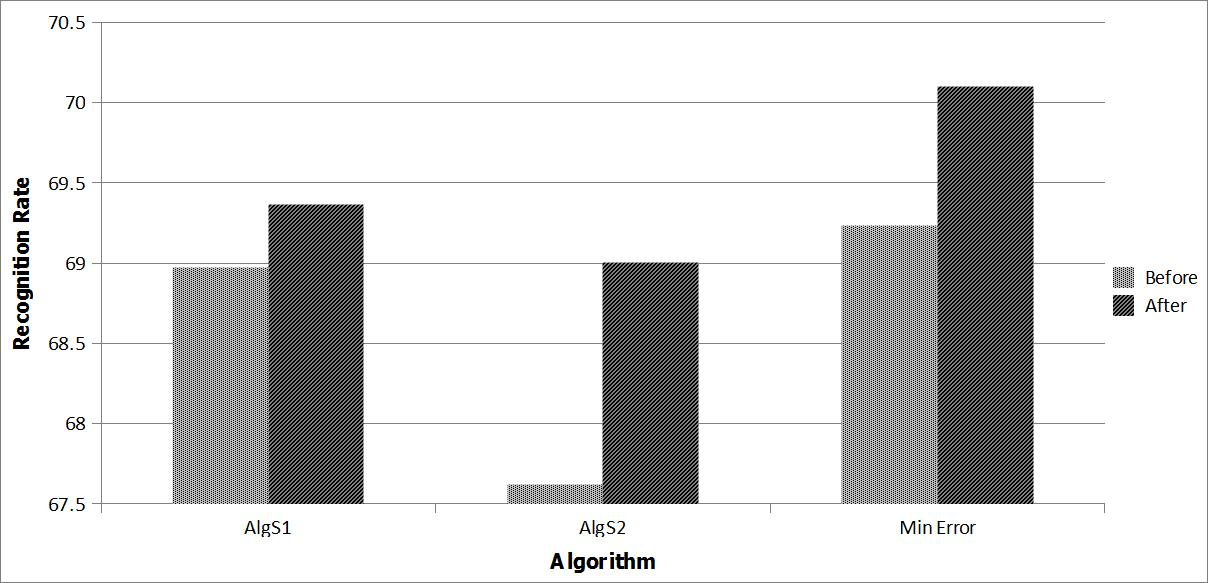
\includegraphics[width=4in]{Experiment68.jpg}
  \caption[Close up of \textit{Hemidactylus} sp.]%
  {Close up of \textit{Hemidactylus} sp., which is
   part the genus of the gecko family. It is the
   second most speciose genus in the family.}
   \label{exp1}
\end{figure}
   \begin{figure}
  \centering
  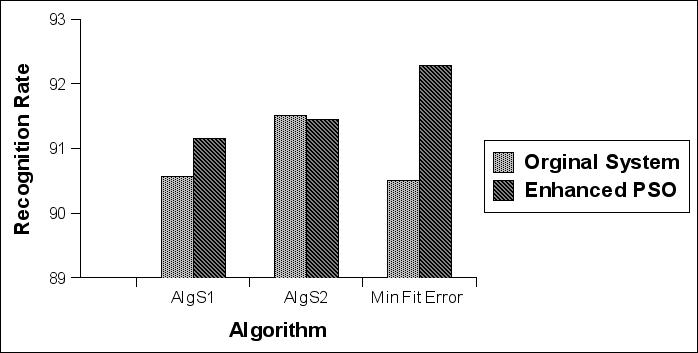
\includegraphics[scale=0.5]{Experiment92.jpg}
  \caption[Close up of \textit{Hemidactylus} sp.]%
  {Close up of \textit{Hemidactylus} sp., which is
   part the genus of the gecko family. It is the
   second most speciose genus in the family.}
   \label{exp2}
\end{figure}
 We performed two experiments to test the system. Firstly, we tested recognition accuracy of shapes in the data set with both algorithms (\textsl{AlgS1} and \textsl{AlgS2}). We also implemented the segmentation algorithm described in \cite{earlyprocess} (\textsl{Alg3}) to compare it with our swarm algorithms. Figure \ref{fig:test1} shows the accuracy achieved by each algorithm. The result shows that (\textsl{AlgS2}) gives better performance than Alg3 and AlgS1. 
 
 
  
\section{Conclusion and Future Work}
 

The training and testing performance measurements using both PSO and Enhanced-PSO in training and testing phases are shown in table (1)

Table 1:- S P measurement performance using both PSO and Enhanced-PSO
We have studied the shape of the sigmoid weight of the hidden layer neurons as a parameter which was usually determined using trial and error. Thus, we add additional parameter called sigmoid weight to the hidden layer neurons to approximate the required non linear dynamical mapping more precisely. We prove that our proposed neural network architecture is a dynamical one because it could be represented by a dynamical nonlinear mapping function. Also, we introduce a new enhanced particle Swarm Optimization method for adjusting
weights of this new proposed neural network architecture based on random perturbation of the particles instead of the standard cognitive term. We prove that our proposed (SDRNN-EPSO) architecture could efficiently give better prediction accuracy and enhanced performance compared to using the SDRNN trained by the Basic-PSO
For the future work, it is suggested that this new enhanced architecture will be used in other different applications of time series prediction and also extended to be used in other applications rather than time series prediction such as pattern recognition and speech verification



This paper presented a new approach to sketch recognition using DPSO. Results show that the \textit{DPSO} in general generates an optimized stroke segmentation which improves the final recognition rate.  The final recognition is based on geometrical, statistical and structural features. The experiments evaluated two \textit{DPSO} different segmentation algorithms (AlgS1 and AlgS2) on simple presentation set dataset. Results show that AlgS2 achieves better segmentation and final accuracy than Alg3 \cite{earlyprocess} on the dataset used. The results proved that the system is easily expandable to more and more symbol as it does not depend on low level primitive recognizers but on high level symbol and geometrical features.  The system achieved an average overall improvement of more than 2\% over Alg3.  


This paper presented a new approach to sketch recognition using PSO. The system uses both speed and curvature information which help improving the \textit{DPSO}. It is noted that the \textit{DPSO} in general generates an optimized stroke segmentation which improves the final recognition rate.  The tradeoff between accuracy achieved and time complexity must be further investigated to achieve better results. The use of statistical moments and structural features improves the recognition rate. The system was tested on 13 different symbols and achieved an accuracy of 91.5\%. The system does not depend on low level recognizer but rather on a set of high level features. This makes the system easily expandable to more and more symbols. 

 A possible extension of this research is to complete the clustering algorithm for fully automated sketch recognition. Currently, the system process one symbol at a time, an enchantment would be to allow users to draw more than one symbol at a time and incorporate a method for separating symbols. Other area of enhancements is the features extraction methods. Introducing more spatial and geometrical features is believed to improve classifications.  


\bibliographystyle{IEEEbib}
\bibliography{../../../neededfiles/Bibliographies/Mybibliography}

\end{document}
